 \documentclass{beamer}
    \usepackage[utf8]{inputenc}
    
    \usetheme{Madrid}
    \usecolortheme{default}
    \usepackage{amsmath,amssymb,amsfonts,amsthm}
    \usepackage{mathtools}
    \usepackage{txfonts}
    \usepackage{tkz-euclide}
    \usepackage{listings}
    \usepackage{adjustbox}
    \usepackage{array}
    \usepackage{gensymb}
    \usepackage{tabularx}
    \usepackage{gvv}
    \usepackage{lmodern}
    \usepackage{circuitikz}
    \usepackage{tikz}
    \lstset{literate={·}{{$\cdot$}}1 {λ}{{$\lambda$}}1 {→}{{$\to$}}1}
    \usepackage{graphicx}
    
    \setbeamertemplate{page number in head/foot}[totalframenumber]
    
    \usepackage{tcolorbox}
    \tcbuselibrary{minted,breakable,xparse,skins}
    
    
    
    \definecolor{bg}{gray}{0.95}
    \DeclareTCBListing{mintedbox}{O{}m!O{}}{%
      breakable=true,
      listing engine=minted,
      listing only,
      minted language=#2,
      minted style=default,
      minted options={%
        linenos,
        gobble=0,
        breaklines=true,
        breakafter=,,
        fontsize=\small,
        numbersep=8pt,
        #1},
      boxsep=0pt,
      left skip=0pt,
      right skip=0pt,
      left=25pt,
      right=0pt,
      top=3pt,
      bottom=3pt,
      arc=5pt,
      leftrule=0pt,
      rightrule=0pt,
      bottomrule=2pt,
      toprule=2pt,
      colback=bg,
      colframe=orange!70,
      enhanced,
      overlay={%
        \begin{tcbclipinterior}
        \fill[orange!20!white] (frame.south west) rectangle ([xshift=20pt]frame.north west);
        \end{tcbclipinterior}},
      #3,
    }
    \lstset{
        language=C,
        basicstyle=\ttfamily\small,
        keywordstyle=\color{blue},
        stringstyle=\color{orange},
        commentstyle=\color{green!60!black},
        numbers=left,
        numberstyle=\tiny\color{gray},
        breaklines=true,
        showstringspaces=false,
    }
    %------------------------------------------------------------
    %This block of code defines the information to appear in the
    %Title page
    \title %optional
    {5.8.25}
    \date{29 September, 2025}
    %\subtitle{A short story}
    
    \author % (optional)
    {INDHIRESH S - EE25BTECH11027}
    
    \begin{document}
    
    \frame{\titlepage}
    
    \begin{frame}{Question}
    One says, "Give me a hundred, Friend! I shall then become twice as rich as you ". The other "if you give me ten, i shall be six times as rich as you ". Tell me What is the amount of their (respective) capital? [From the bijaganita of Bhaskara II].
    \end{frame}
    
    \begin{frame}[allowframebreaks] 
    \frametitle{Equation}
        \centering
        \label{tab:parameters}
   Let an amount with Friend 1 be $a$ and amount with Friend 2 be $b$\\
From given information:
\begin{align}
   a+100=2(b-100)
\end{align}
\begin{align}
 a-2b=-300
\end{align}
And
\begin{align}
  b+10=6(a-10)
 \end{align}

\begin{align}
   b+10=6a-60;
\end{align}

\begin{align}
    6a-b=70
\end{align}
    \end{frame}
    
    \begin{frame}
    \frametitle{Theoretical Solution}
   By combining the Eq.2 and Eq.5 we get
\begin{align}
  \myvec{1&-2\\6&-1}\Vec{x}=\myvec{-300\\70}
\end{align}
Where
\begin{align}
\Vec{x}=\myvec{a\\b}
\end{align}
\begin{align}
     \augvec{2}{1}{1 & -2 & -300\\6 & -1 & 70} \xleftrightarrow{R_2\longleftarrow R_2-6R_1} \augvec{2}{1}{1 & -2 & -300\\0 & 11 & 1870}
\end{align}
\begin{align}
    \augvec{2}{1}{1 & -2 & -300\\0 & 11 & 1870} \xleftrightarrow{R_2\longleftarrow \frac{1}{11}R_2} \augvec{2}{1}{1 & -2 & -300\\0 & 1 & 170}
\end{align}

    \end{frame}
    
    \begin{frame}
    \frametitle{Theoretical solution}
   \begin{align}
   \augvec{2}{1}{1 & -2 & -300\\0 & 1 & 170} \xleftrightarrow{R_1\longleftarrow R_1+2R_2} \augvec{2}{1}{1 & 0 & 40\\0 & 1 & 170}
\end{align}
\begin{align}
    \Vec{x}=\myvec{40\\170}
\end{align}

\begin{align}
a=40\;\;and\;\;b=170
  \end{align}
The amount with Friend 1 = 40 \\
The amount with Friend 2 = 170
    \end{frame}
    
    
    \begin{frame}[fragile]
        \frametitle{C Code}
        \begin{lstlisting}
  typedef struct {
    double a;
    double b;
} Solution;

Solution solve_equations(double a1, double b1, double c1, double a2, double b2, double c2) {
    Solution sol;
    double determinant = a1 * b2 - a2 * b1;

    // Use Cramer's rule to find 'a' and 'b'
    if (determinant != 0) {
        sol.a = (c1 * b2 - c2 * b1) / determinant;
        sol.b = (a1 * c2 - a2 * c1) / determinant;
    } 
        \end{lstlisting}
    \end{frame}
    
 \begin{frame}[fragile]
        \frametitle{C Code}
        \begin{lstlisting}
 else {
        // Fallback for singular matrix
        sol.a = 0.0;
        sol.b = 0.0;
    }
    return sol;
}
        \end{lstlisting}
    \end{frame}
    
    \begin{frame}[fragile]
        \frametitle{Python Code}
        \begin{lstlisting}
import os
import ctypes
import numpy as np
import matplotlib.pyplot as plt

# --- Hardcoded inputs from the question ---
a1, b1, c1 = 1, -2, -300
a2, b2, c2 = 6, -1, 70

# --- Compile and Load C Library ---
if os.system("gcc -shared -o word.so -fPIC word.c") != 0:
    print("\nC compilation failed. Exiting.")
    exit()

class Solution(ctypes.Structure):
    _fields_ = [("a", ctypes.c_double), ("b", ctypes.c_double)]


        \end{lstlisting}
    \end{frame}
    
    \begin{frame}[fragile]
        \frametitle{Python Code}
        \begin{lstlisting}
c_lib = ctypes.CDLL(os.path.abspath("word.so"))
c_lib.solve_equations.argtypes = [ctypes.c_double] * 6
c_lib.solve_equations.restype = Solution

# --- Solve by Calling C Function ---
solution = c_lib.solve_equations(a1, b1, c1, a2, b2, c2)
a_sol, b_sol = solution.a, solution.b
print(f"Solution from C: a = {a_sol:.2f}, b = {b_sol:.2f}")

# --- Plot the Graph ---
a_vals = np.linspace(a_sol - 50, a_sol + 50, 400)
b1_vals = (c1 - a1 * a_vals) / b1
b2_vals = (c2 - a2 * a_vals) / b2

plt.figure(figsize=(10, 8))
plt.plot(a_vals, b1_vals, label=f'{a1}a + {b1}b = {c1}')
plt.plot(a_vals, b2_vals, label=f'{a2}a + {b2}b = {c2}')


        \end{lstlisting}
    \end{frame}
    
    \begin{frame}[fragile]
        \frametitle{Python Code}
        \begin{lstlisting}
    # Mark the intersection
plt.scatter(a_sol, b_sol, color="red", s=200, marker="*", edgecolors="black",
            label=f'Intersection ({a_sol:.0f}, {b_sol:.0f})')

# Annotate with arrow
plt.annotate(f"({a_sol:.0f}, {b_sol:.0f})",
             (a_sol, b_sol),
             textcoords="offset points",
             xytext=(10,10),
             fontsize=12,
             color="red",
             arrowprops=dict(arrowstyle="->", color="red"))


        \end{lstlisting}
    \end{frame}
    
    \begin{frame}[fragile]
        \frametitle{Python Code}
        \begin{lstlisting}
   plt.title("Graphical Solution of Linear Equations", fontsize=16)
plt.xlabel("a-axis", fontsize=12)
plt.ylabel("b-axis", fontsize=12)
plt.grid(True)
plt.legend()
plt.savefig("/media/indhiresh-s/New Volume/Matrix/ee1030-2025/ee25btech11027/MATGEO/5.8.25/figs/figure1.png")
plt.show()
        \end{lstlisting}
    \end{frame}
    
    \begin{frame}{Plot}
        \begin{center}
            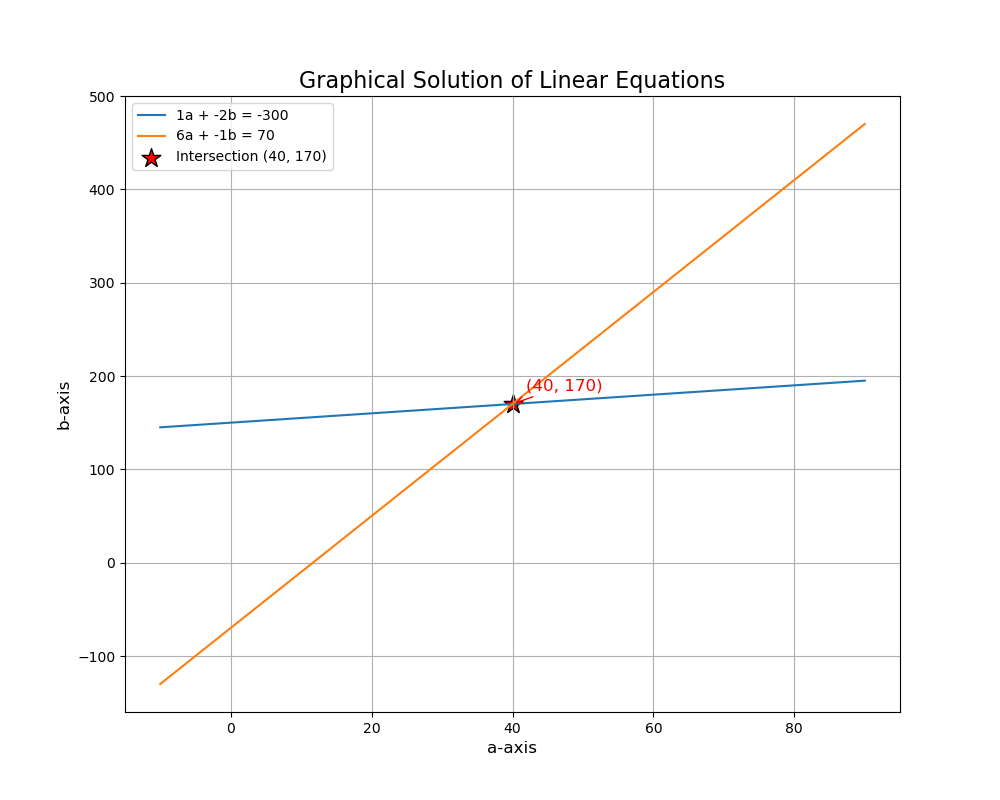
\includegraphics[width=\columnwidth, height=0.8\textheight, keepaspectratio]{figs/figure1.png}
        \end{center}
    \end{frame}
    
    \end{document}